\chapter{Abordagem Proposta}
\label{cap:abordagem_proposta}

Para o desenvolvimento deste trabalho, propõe-se cinco etapas principais que seguem a estrutura padrão adotada pelos trabalhos analisados, conforme ilustrado na Figura \ref{fig:abordagemPadrao}. Inicialmente, é realizada a construção do conjunto de dados, cujos processos são descritos em detalhes na Seção \ref{sec:base_dados}. Em seguida, ocorre a seleção de variáveis relevantes, abordada na Seção \ref{sec:selecao_variaveis}. Com as variáveis selecionadas, inicia-se o processo de previsão, que é detalhado na Seção \ref{sec:previsao}. Por fim, é realizada a recomendação de investimento com base nos valores previstos, conforme descrito na Seção \ref{sec:estrategia}. 


\section{Base de Dados}
\label{sec:base_dados}
O processo de construção da base de dados é dividido em duas etapas distintas. Primeiramente, ocorre a extração dos dados, conforme detalhado na Seção \ref{subsec:extracao}. Em seguida, é realizada a geração de novas variáveis a partir dos dados extraídos, como explicado na Seção \ref{subsec:feature_generate}. Nessa fase, são criadas variáveis adicionais que fornecem informações relevantes para o processo de previsão e análise. A Figura \ref{fig:base_dados} apresenta uma visão geral do processo de construção da base de dados, ilustrando de forma visual as etapas mencionadas. Esse processo garante a disponibilidade dos dados necessários e a preparação adequada das variáveis para as etapas subsequentes do trabalho.

\begin{figure}[htbp]
    \caption{Visão macro do processo de construção da base da dados.}
      \centering
    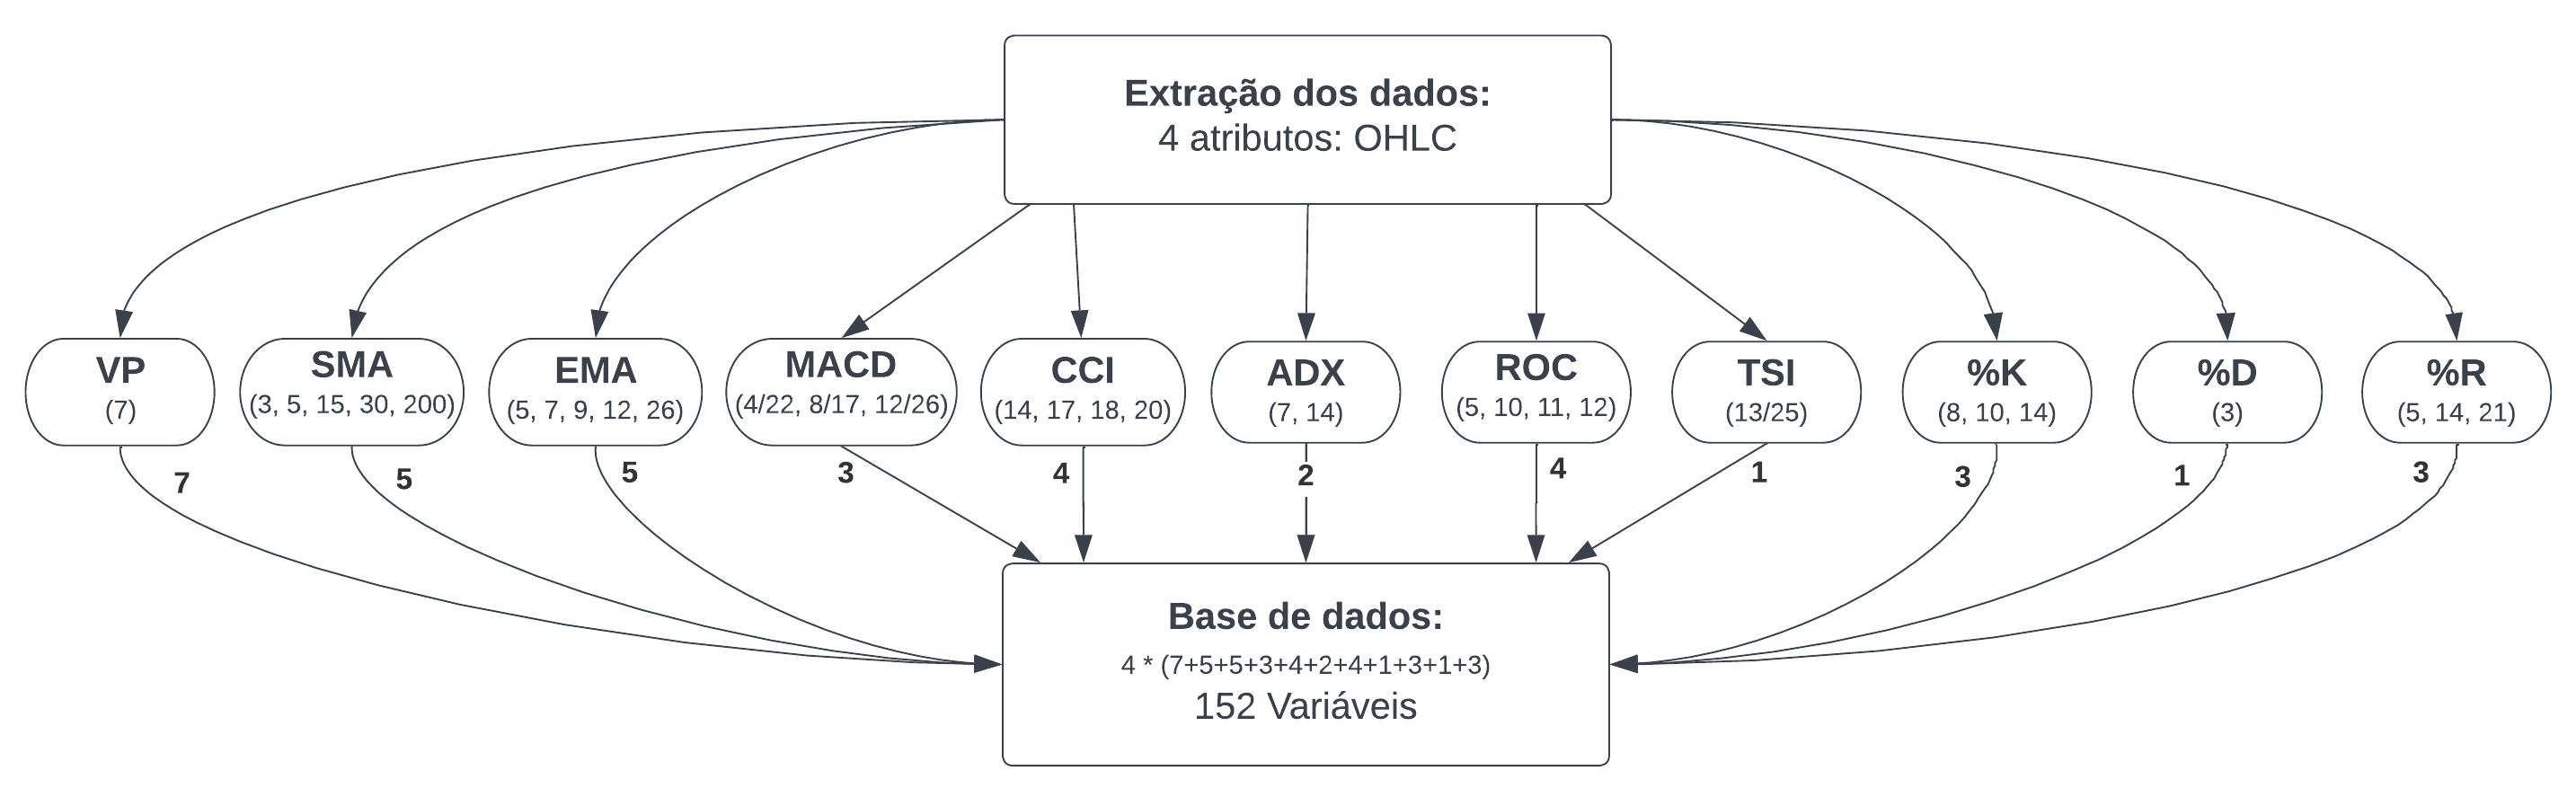
\includegraphics[width=.99\linewidth]{sections/images/base_dados.png} 
    \label{fig:base_dados}
\end{figure}


\subsection{Extração}
\label{subsec:extracao}
O mercado de ações do Brasil opera de segunda a sexta-feira, das 10:00 às 17:00 \cite{B3H:2023}. Durante esse período, são geradas informações em diversas granularidades, permitindo acompanhar a evolução dos preços e volumes de negociação ao longo do tempo. Uma plataforma amplamente utilizada para acessar essas informações é a plataforma \textit{Investing} \footnote{http://www.investing.com}, que disponibiliza dados históricos e em tempo real em diferentes intervalos, como diário, semanal e mensal. Além disso, essa plataforma abrange diversos mercados e modalidades de investimento em vários países, fornecendo informações relevantes, como os preços de \ac{OHLC}, volume negociado e percentual de mudança. No contexto deste trabalho, os dados históricos de \ac{OHLC} foram extraídos dessa plataforma para análise e estudo.

\subsection{Geração de novas Variáveis}
\label{subsec:feature_generate}
Após a extração dos dados, são aplicadas diversas técnicas para gerar novas variáveis relevantes na tarefa de previsão do preço de fechamento da próxima amostra. Para isso, são calculadas novas \textit{features} para cada valor de \ac{OHLC}, empregando-se diversas fórmulas estatísticas, como:
\begin{itemize}
    \item \ac{VP} - é obtido realizando o deslocamento de valores passados. Neste estudo, utiliza-se um deslocamento de 7 valores passados \cite{Vinicius_Sistemas}.

    \item \ac{SMA} - calculado a partir da Equação (\ref{eq:SMA}). No presente estudo, utilizaram-se os intervalos de 3 \cite{chantarakasemchit2020forex}, 5, 15, 30 \cite{handayani2019longer} e 200 \cite{ELLIS2005399}.
    
    \item \ac{EMA} - tem seu calculo baseado na Equação (\ref{eq:EMA}). Neste estudo, foram adotados os períodos amostrais de 5, 7, 9 \cite{ANBALAGAN2015214}, 12 \cite{Charlene} e 26 \cite{ananthi2021retracted}.
    
    \item \ac{MACD} - derivado da Equação (\ref{eq:MACD}). Nesta pesquisa, foram utilizados os valores de janela móvel curta e janela móvel longa como 12/26 \cite{ANBALAGAN2015214, handayani2019longer}, 8/17 e 4/22 \cite{kang2021improving}, respectivamente.
    
    \item \ac{CCI} - calculado a partir da Equação (\ref{eq:CCI}). Neste trabalho, foram considerados os períodos de amostragem de 14 \cite{halil2019predicting}, 17, 18 \cite{karasu2022crude} e 20 \cite{kelotra2020stock} para a janela de análise.
    
    \item \ac{ADX} - obtido através da aplicação da Equação (\ref{eq:ADX}). Este estudo considera os períodos de 7 \cite{kelotra2020stock} e 14 \cite{shamseddin2022mapping} espaços amostrais.
    
    \item \ac{ROC} - determinado a partir da equação (\ref{eq:ROC}). O presente estudo adota os intervalos de 5, 10, 11 e 12 \cite{karasu2022crude} para o calculo do mesmo.
    
    \item \ac{TSI} - calculado utilizando a Equação (\ref{eq:TSI}). Neste experimento, são adotados os intervalos de 13 para a janela móvel curta e 25 para a janela móvel longa \cite{nayak2015naive, anwar2019forecasting}.
    
    \item \ac{K} - calculado com base na Equação (\ref{eq:K}). Neste estudo, são utilizados os intervalos de tempo de 8 \cite{ni2022does}, 10 \cite{ijegwa2014predictive} e 14 amostras \cite{C_Veeramani_Exploration}.
    
    \item \ac{D} - derivado da Equação (\ref{eq:D}). No presente trabalho, adotou-se a janela de tempo de 3 amostras \cite{ijegwa2014predictive, vaidya2018stochastic}.
    
    \item \ac{R} - tem seu calculo baseado na Equação (\ref{eq:R}). Neste estudo, são consideradas as janelas de tempo de 5, 14 e 21 espaços amostrais \cite{de2016multi}.
    
\end{itemize}
Como resultado desse processo, são geradas um total de 152 novas variáveis, o que proporciona uma variedade de padrões de entrada para os modelos de predição.



\section{Seleção de Variáveis}
\label{sec:selecao_variaveis}
Com a base de dados gerada, é importante destacar que nem todas as variáveis possuem igual relevância para o processo de previsão. Portanto, é necessário realizar a seleção de variáveis, a qual foi dividida em duas etapas neste trabalho. Primeiramente, são aplicados métodos de seleção de variáveis descritos na Seção \ref{subsec:selecao_variaveis}. Em seguida, ocorre a fusão de todas as variáveis selecionadas e a classificação delas em dois conjuntos de dados distintos, denominados \textit{Dataset-1} e \textit{Dataset-2}. Uma representação geral desse processo pode ser visualizada na Figura \ref{fig:feature_selection}.

\begin{figure}[htbp]
    \caption{Visão macro do processo de seleção de variáveis.}
      \centering
    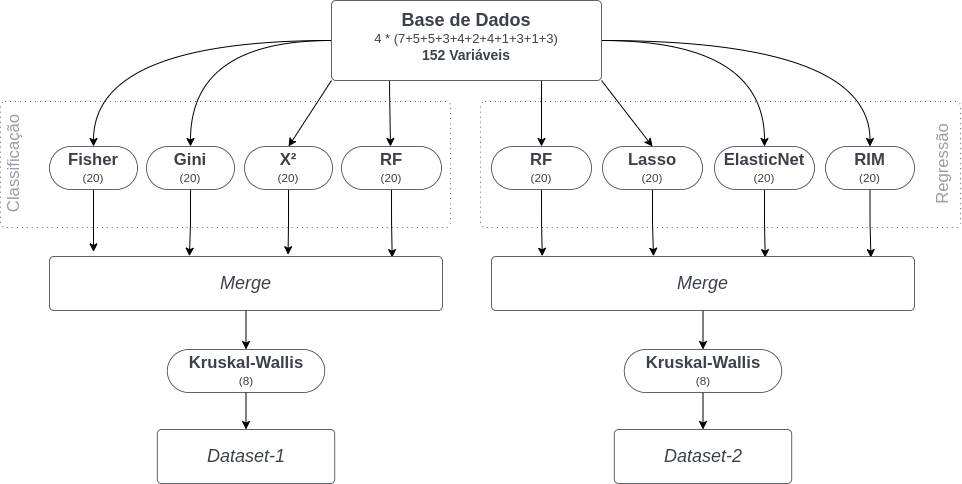
\includegraphics[width=.99\linewidth]{sections/images/feature_selection.png} 
    \label{fig:feature_selection}
\end{figure}

Na primeira etapa do processo de seleção de variáveis, são aplicados dois grupos de algoritmos. O primeiro grupo é direcionado para modelos de classificação e inclui os métodos de Fisher, Gini, \ac{R2} e \ac{RF}. Já o segundo grupo é direcionado para modelos de regressão e inclui os métodos de \ac{RF}, Lasso, ElasticNet e \ac{RIM}. Cada um desses métodos, pertencentes aos dois grupos, seleciona 20 atributos relevantes para a classificação ou regressão, respectivamente. 

Por fim, na segunda etapa do processo de seleção de variáveis, é realizado um \textit{merge} em cada grupo, unificando as variáveis selecionadas por cada algoritmo, sem que haja repetição. Em seguida, é aplicado o teste de \textit{Kruskal-Wallis} em cada grupo para ranquear as variáveis mais relevantes provenientes do \textit{merge}. Isso resulta em dois conjuntos de dados com 8 variáveis cada: o \textit{Dataset-1}, referente ao grupo de classificação, e o \textit{Dataset-2}, referente ao grupo de regressão. O uso do modelo de \textit{Kruskal-Wallis} permite ordenar as variáveis de acordo com sua relevância, considerando as características específicas de cada grupo. Essa etapa visa consolidar os conjuntos de dados finais, contendo as variáveis mais importantes para cada tipo de modelo, otimizando assim o processo de previsão.




\section{Modelo de Previsão}
\label{sec:previsao}
Para a construção do modelo de previsão proposto, foram utilizadas duas técnicas de \textit{ensemble}: o \textit{Soft Voting} e o \textit{Stacking}.

O \textit{Soft Voting}, como descrito por \citeonline{wang2013soft}, realiza a votação ponderada, expressando a saída em percentuais referentes a cada classe. Nessa técnica, vários modelos são treinados independentemente e suas previsões são combinadas usando pesos. O resultado final é uma média ponderada das previsões de cada modelo, refletindo a confiança de cada modelo na classificação de uma determinada classe.

Já o \textit{Stacking}, introduzido por \citeonline{dietterich2002ensemble}, envolve a criação de camadas de modelos de aprendizado de máquina conectados. Nessa abordagem, os modelos de base são treinados em conjunto, e suas previsões são usadas como entrada para um meta-modelo que realiza a previsão final. O objetivo é combinar as previsões dos modelos de base de forma a obter uma previsão mais acurada.

\begin{figure}[htbp]
    \caption{Visão macro do processo de previsão.}
      \centering
    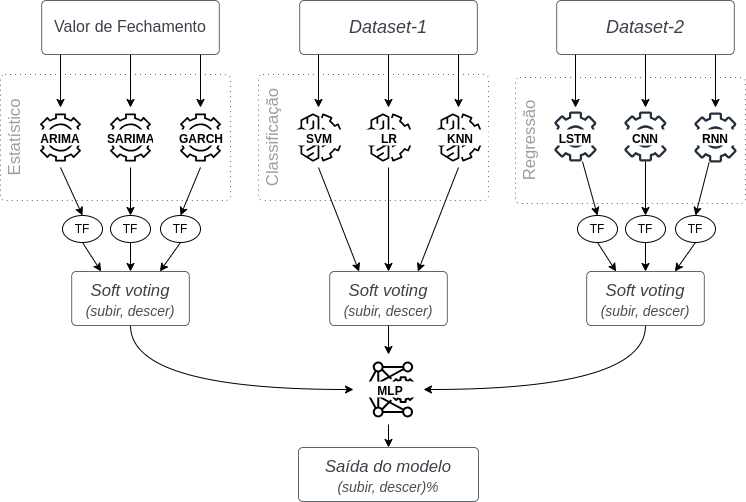
\includegraphics[width=.99\linewidth]{sections/images/model_prediction.png} 
    \label{fig:model_prediction}
\end{figure}

No modelo proposto, são construídos três grupos de algoritmos distintos para realizar as previsões. O primeiro grupo consiste em modelos estatísticos, como \ac{ARIMA}, \ac{SARIMA} e \ac{GARCH}, que utilizam apenas o valor de fechamento de cada amostra como entrada e possuem uma função de transformação na saída de cada modelo, conforme descrita na Tabela \ref{tab:RegraTransf}. O segundo grupo é composto por modelos de \ac{IA} voltados para classificação, como \ac{SVM}, \ac{LR} e \ac{KNN}, que recebem como entrada o \textit{Dataset-1}, composto pelas variáveis relevantes selecionadas para classificação. O terceiro grupo é formado por modelos de \ac{IA} voltados para regressão, como \ac{LSTM}, \ac{RNN} e \ac{CNN}, que recebem como entrada o \textit{Dataset-2}, contendo as variáveis relevantes selecionadas para regressão e também possuem uma função de transformação na saída de cada modelo, de acordo com a Tabela \ref{tab:RegraTransf}. 

Em continuidade, as técnicas de \textit{Soft Voting} e \textit{Stacking} são aplicadas de forma sequencial. O \textit{Soft Voting} combina as previsões de cada grupo de modelos, considerando a contribuição de cada um deles. Isso resulta em uma lista com valores de pertinência para cada classe. Por sua vez, o \textit{Stacking} utiliza uma rede MLP para combinar as saídas do \textit{Soft Voting} de cada grupo, resultando em uma lista de percentuais de correlação a cada classe. Essa abordagem permite aproveitar a diversidade dos modelos utilizados e proporciona uma previsão mais robusta e confiável para a tarefa de classificação.

A proposta do modelo de previsão e a aplicação das técnicas de \textit{ensemble} podem ser visualizadas na Figura \ref{fig:model_prediction}, apresentando a sequência e interconexão dos diferentes estágios do processo.


\section{Recomendação de Investimento}
\label{sec:estrategia}

Tendo em mãos o percentual de subida ou descida previsto pelo modelo proposto, inicia-se o processo de recomendação de compra e venda, conforme ilustrado na a Figura \ref{fig:strategy}, que objetiva reduzir operações de baixa confiabilidade e maximizar os retornos financeiros. A estratégia de recomendação é baseada nos resultados do modelo de previsão, visando identificar oportunidades de investimento com maior probabilidade de sucesso.

\begin{figure}[htbp]
    \caption{Visão macro do processo de recomendação de investimentos.}
      \centering
    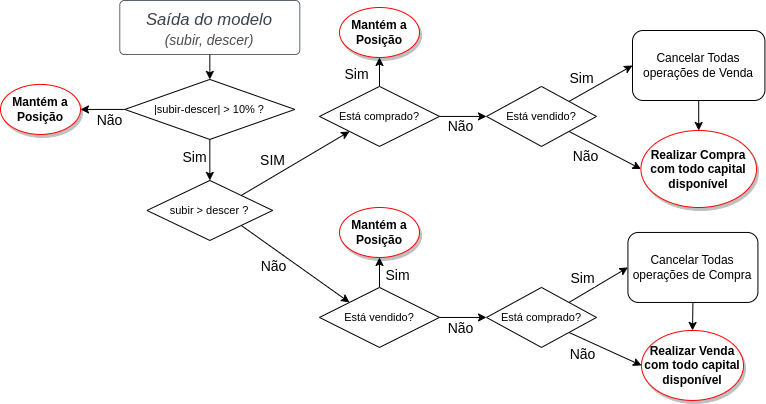
\includegraphics[width=.99\linewidth]{sections/images/strategy.png} 
    \label{fig:strategy}
\end{figure}

A estratégia de recomendação inicia com um filtro para verificar se a diferença percentual entre as classes de subida e descida é relevante. Se a diferença não for significativa, a recomendação é não realizar nenhuma operação e manter a posição atual. Caso a diferença seja relevante, é feita uma comparação para determinar qual classe possui maior percentual de pertinência.

Se o sinal de subida for mais relevante, então é mais provável que o próximo valor seja maior do que o atual. Nesse ponto, é verificado se há uma operação de compra em andamento. Se houver, é recomendado não realizar nenhuma ação. Caso contrário, há uma verificação adicional para determinar se existe alguma operação de venda em andamento. Se houver, é recomendado encerrar todas as operações vigentes e realizar a compra utilizando todo o capital disponível. Se não houver operação de venda em andamento, é recomendado realizar a compra utilizando todo o capital.

Por outro lado, se o sinal de subida não for maior que o de descida, então é mais provável que o próximo valor seja menor do que o atual. Nessa etapa, é verificado se há uma operação de venda em andamento. Se houver, a recomendação é não realizar nenhuma ação. Caso contrário, é feita uma nova verificação para identificar se há uma operação de compra em andamento. Se houver, é recomendado encerrar todas as operações de compra e realizar uma venda utilizando todo o capital disponível. Caso não haja operação de compra em andamento, é recomendado realizar a venda utilizando todo o capital disponível. 





